%aQGC results

All log-likelihood distributions are shown.

\begin{figure}[ht]
    \centering
    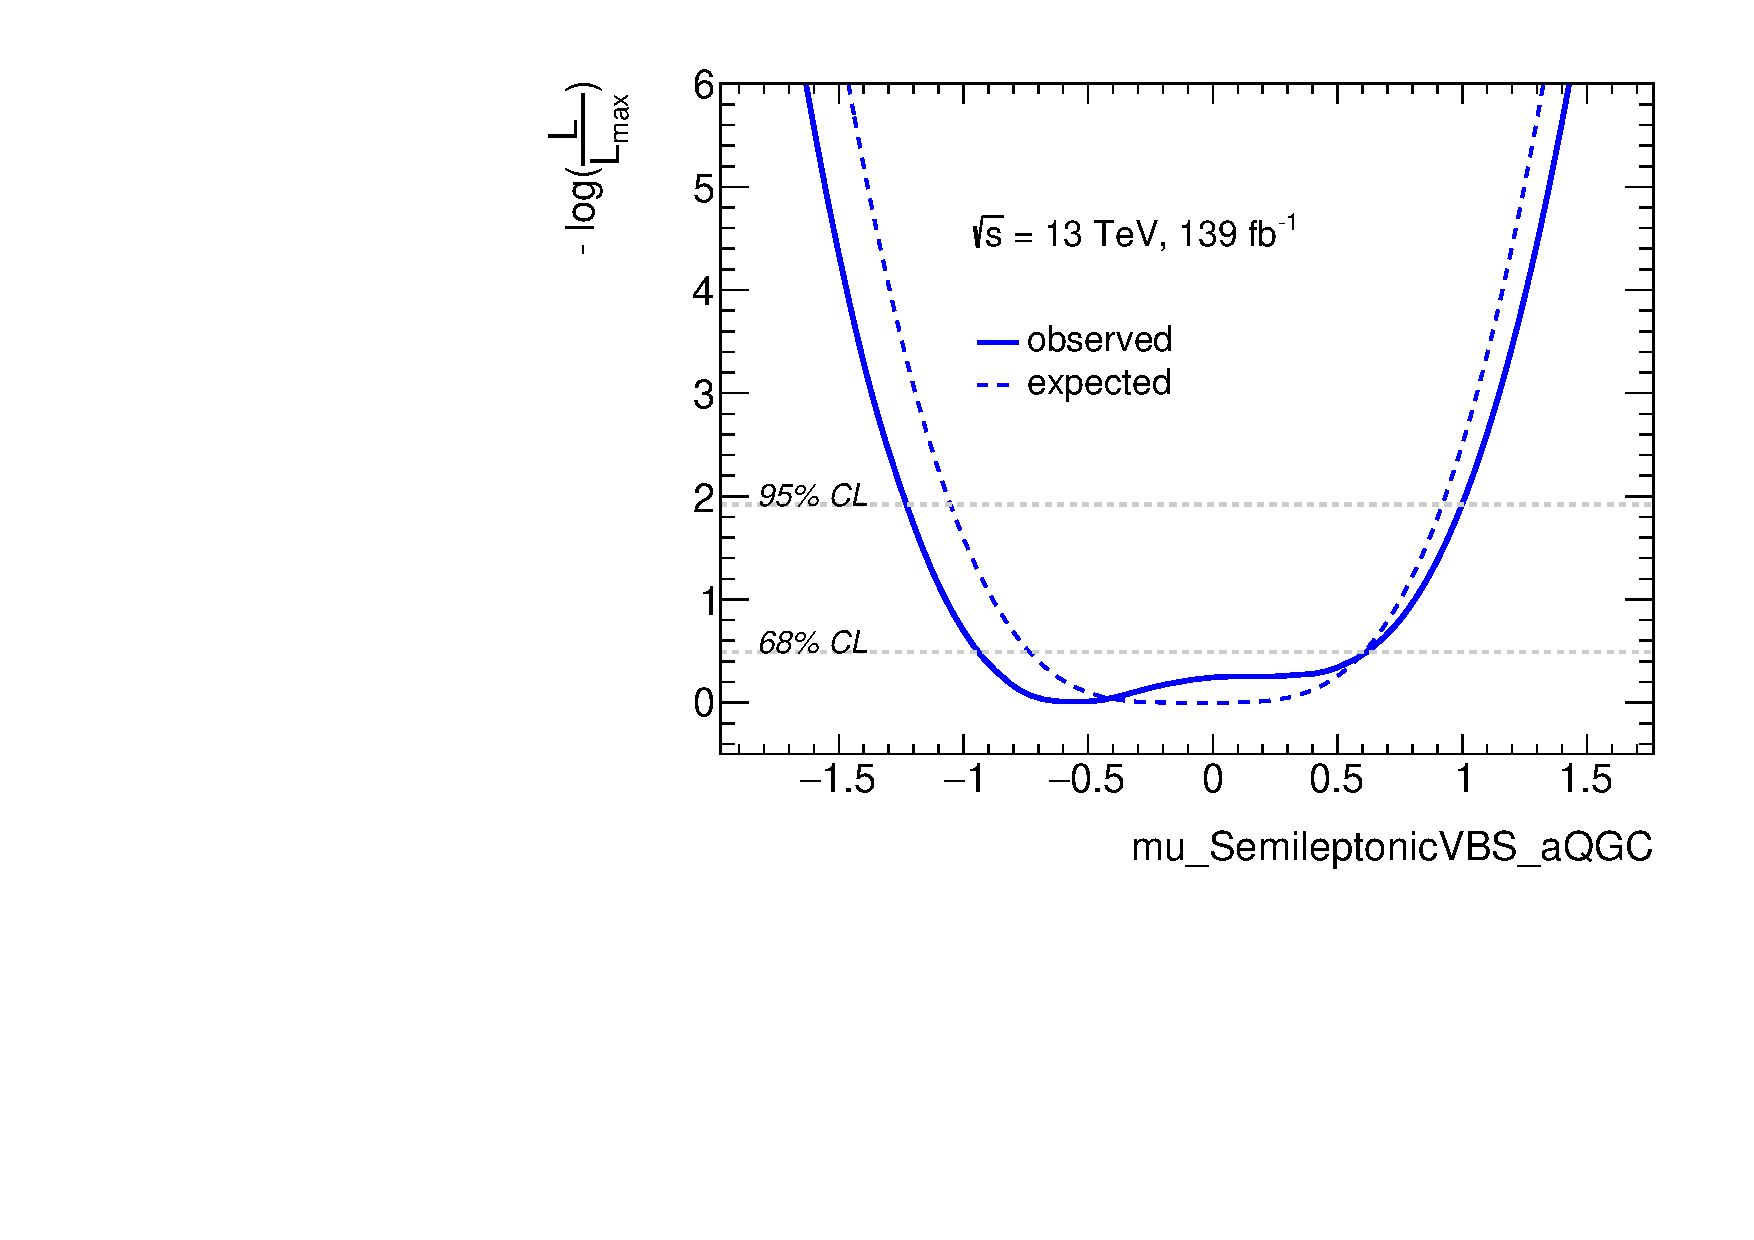
\includegraphics[width=0.32\textwidth]{figures/aQGC/profileFT01500}
    	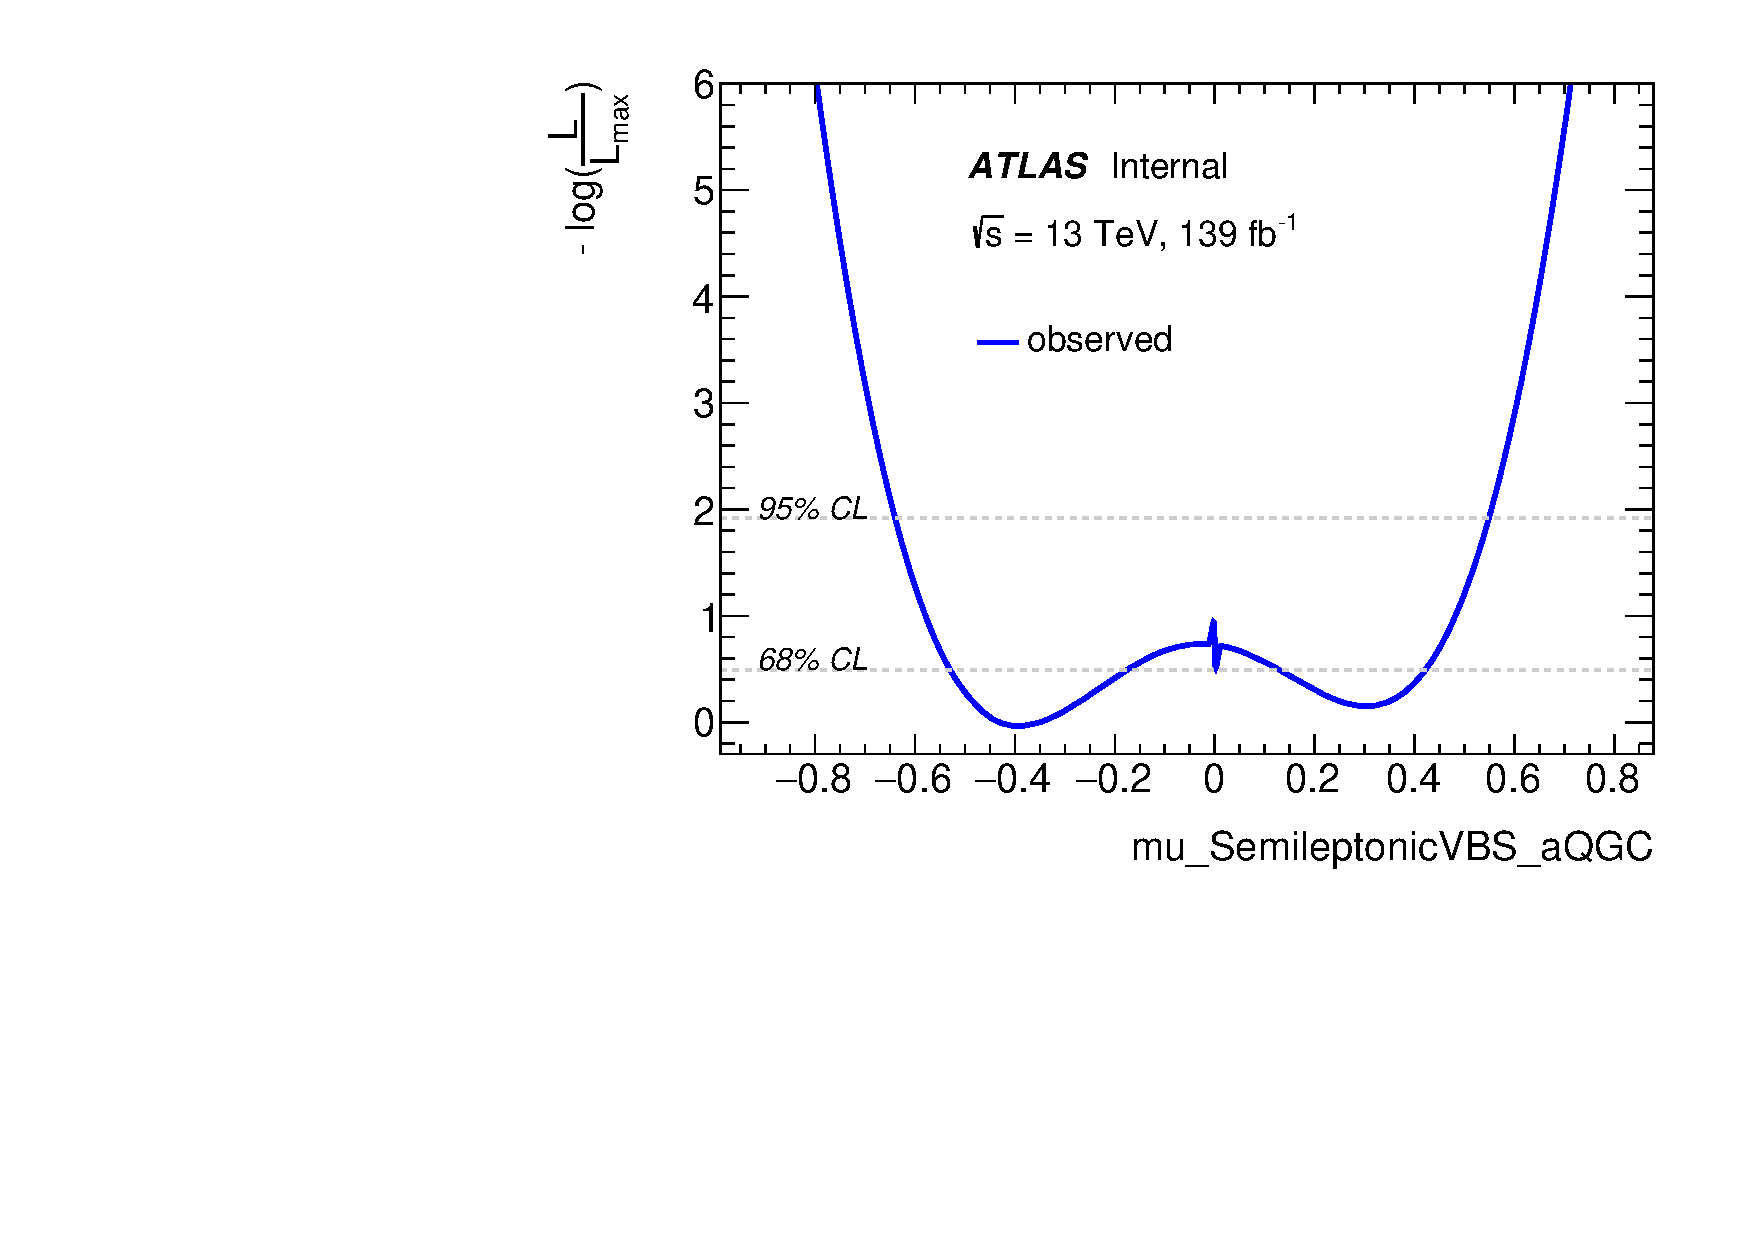
\includegraphics[width=0.32\textwidth]{figures/aQGC/profileFT02000}
    	%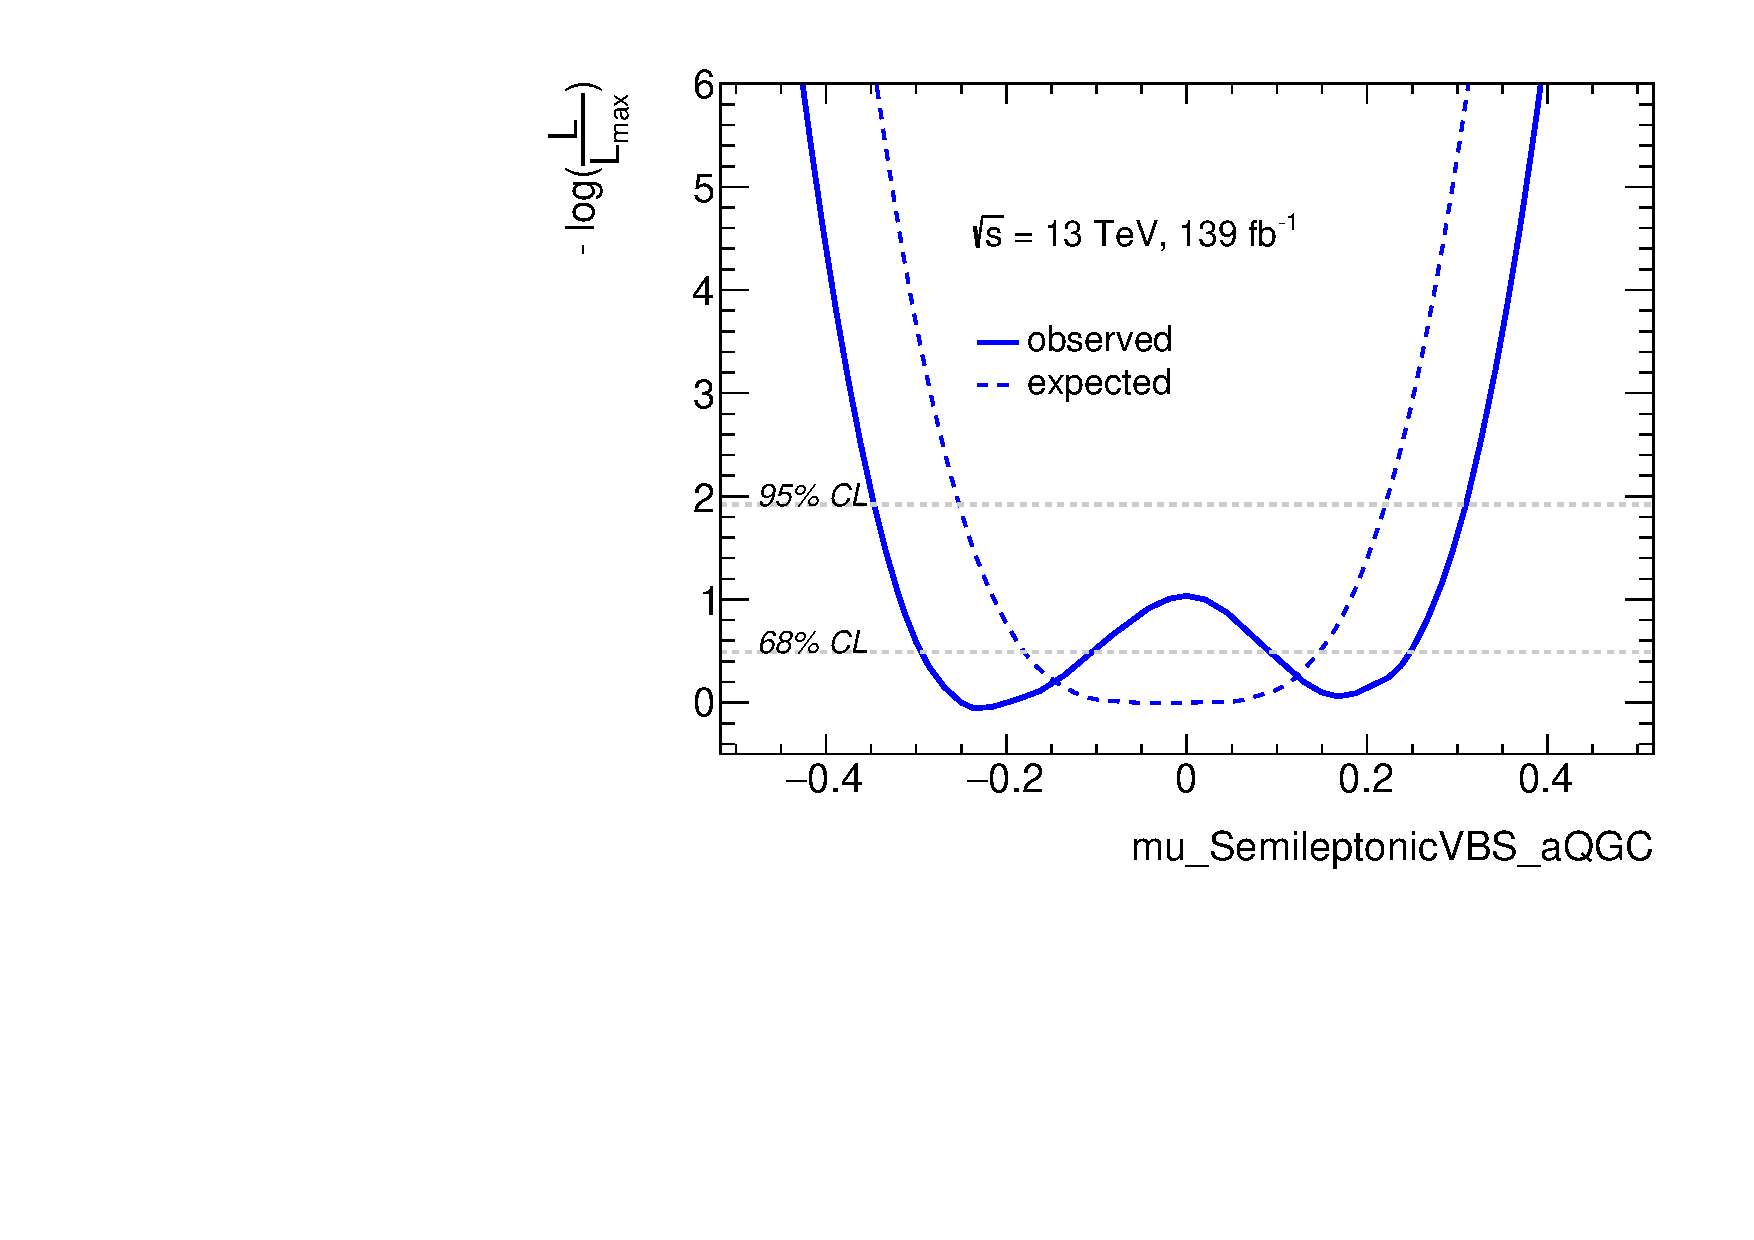
\includegraphics[width=0.38\textwidth]{figures/aQGC/profileFT03000}
        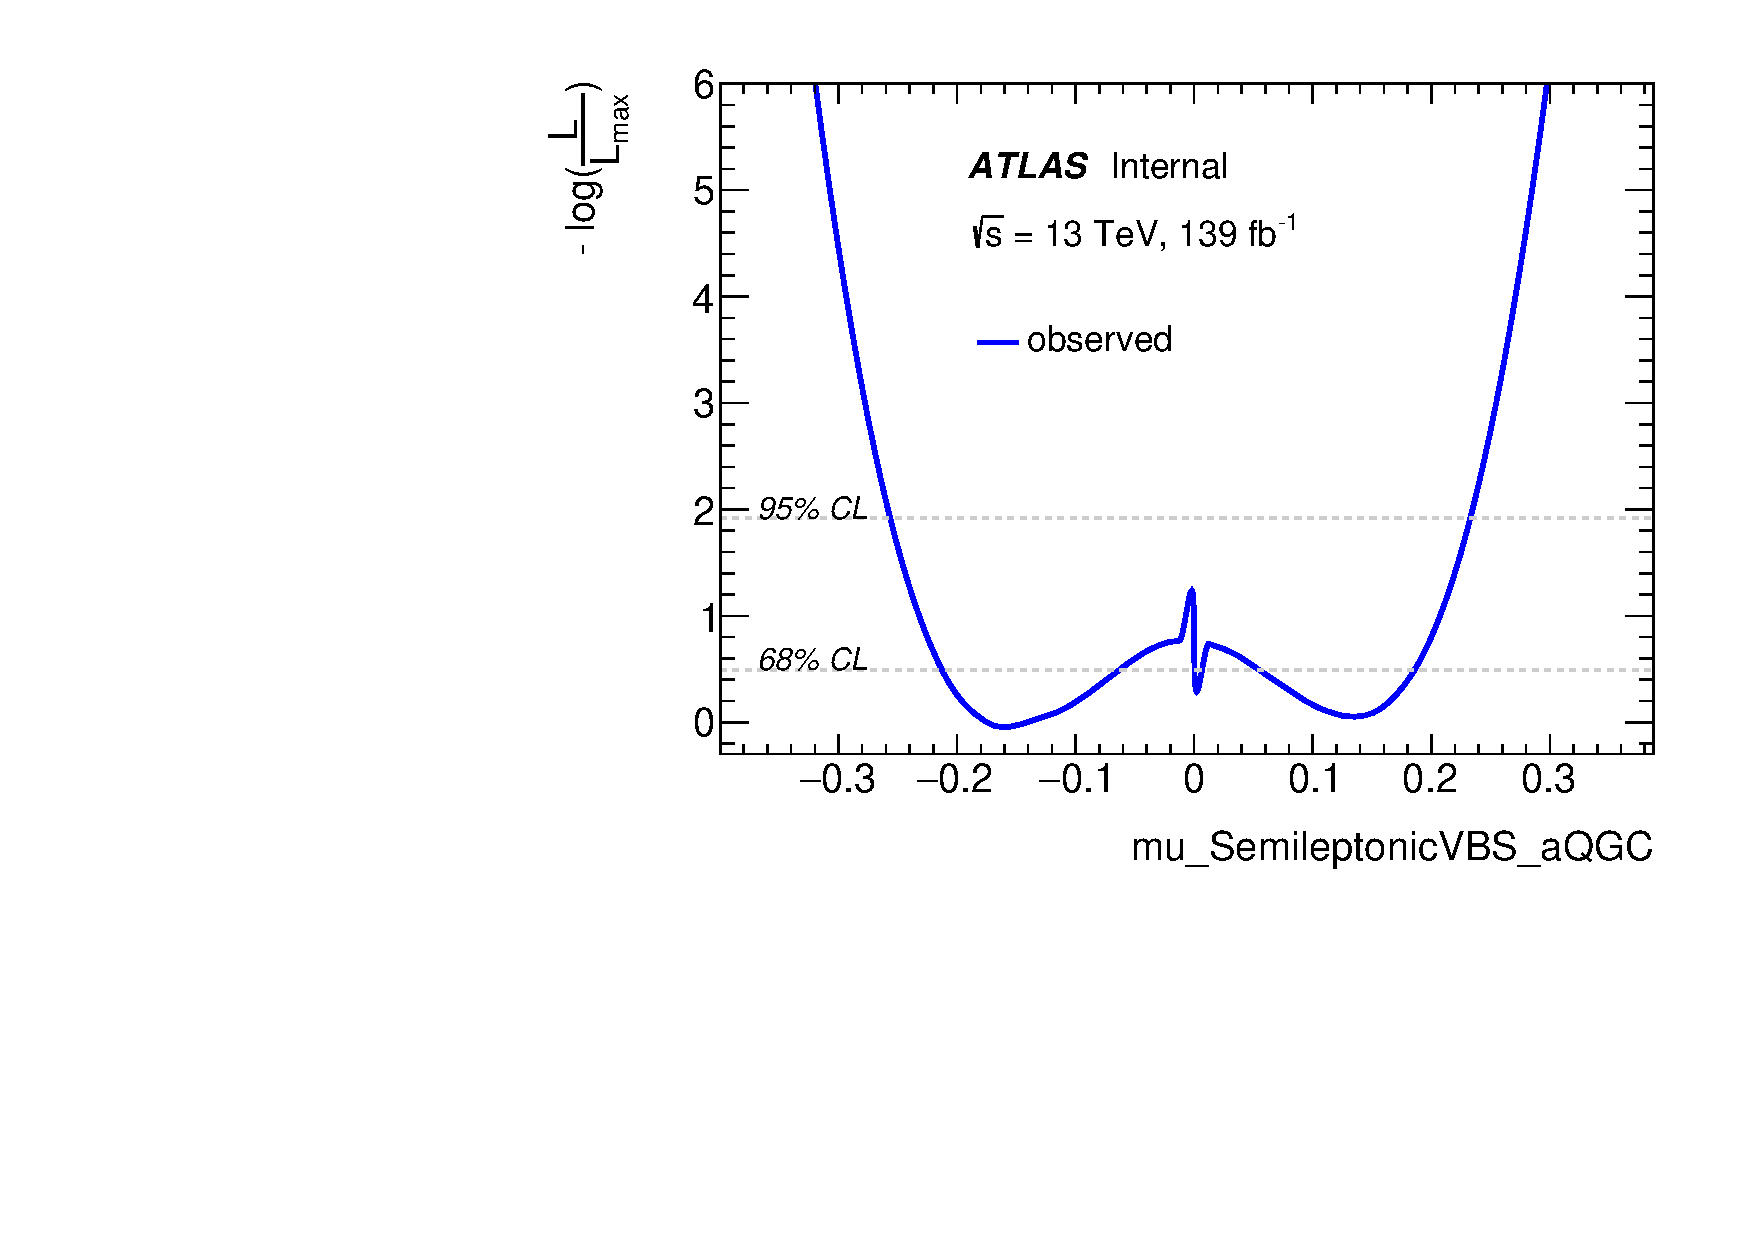
\includegraphics[width=0.32\textwidth]{figures/aQGC/profileFT0inf}
        \caption{The observed log-likelihood curves of FT0 Wilson coefficient where the clipping energy is 1.5~TeV (left), 2.0~TeV (middle), $\infty$ (right).}
        \label{fig:ProfileLL}
\end{figure}



All expected and observed limits are shown.

\begin{figure}[ht]
    \centering
    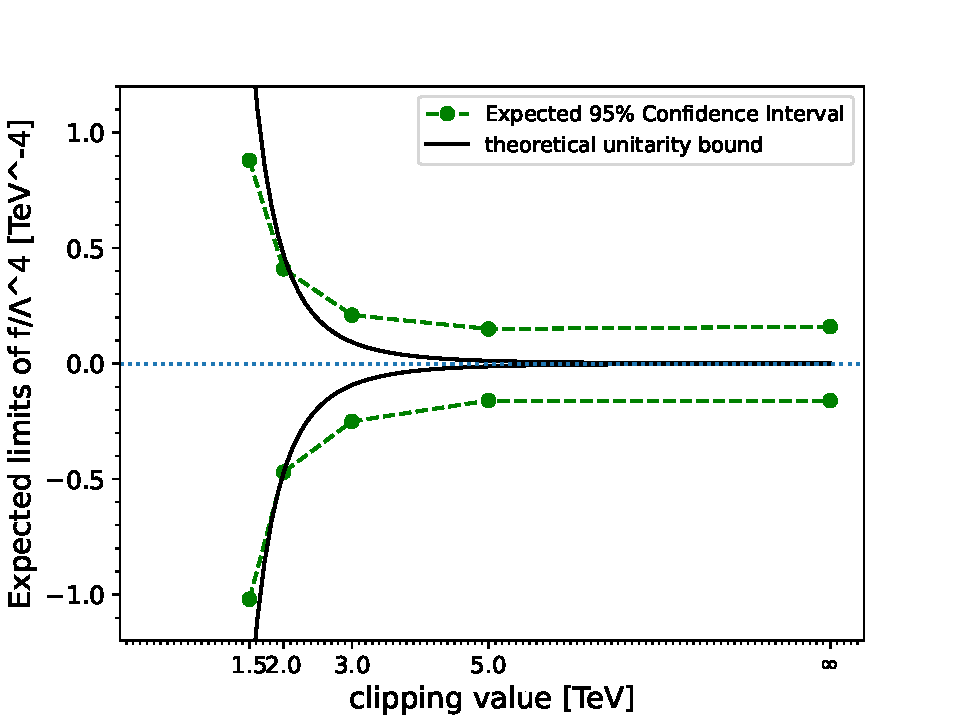
\includegraphics[width=0.45\textwidth]{figures/aQGC/ClippedFT0CI.pdf}
    	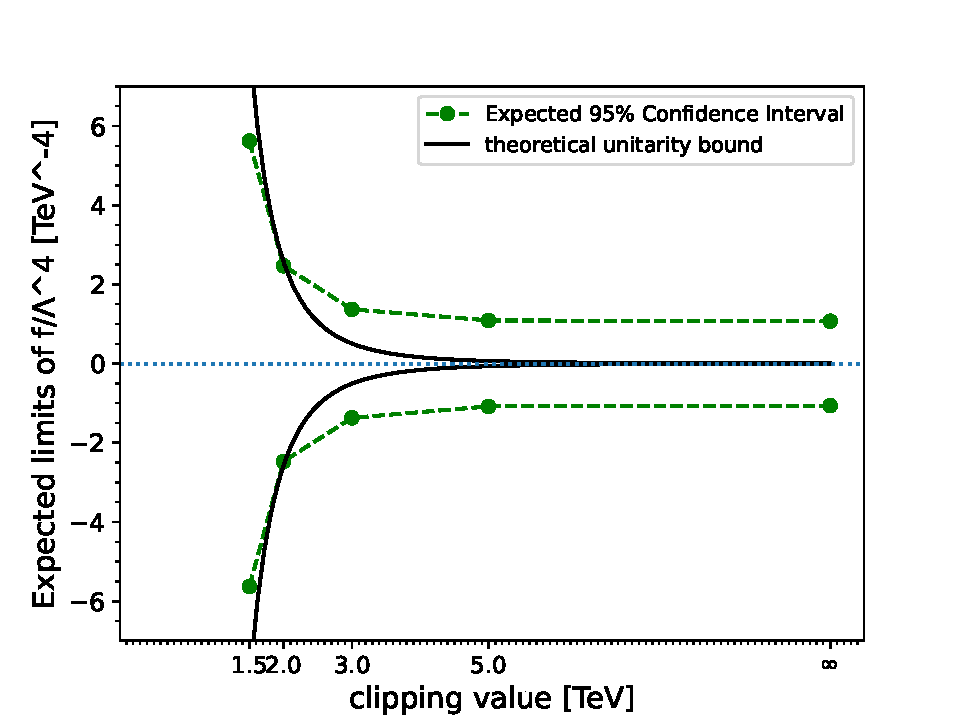
\includegraphics[width=0.45\textwidth]{figures/aQGC/ClippedFM0CI.pdf}
    	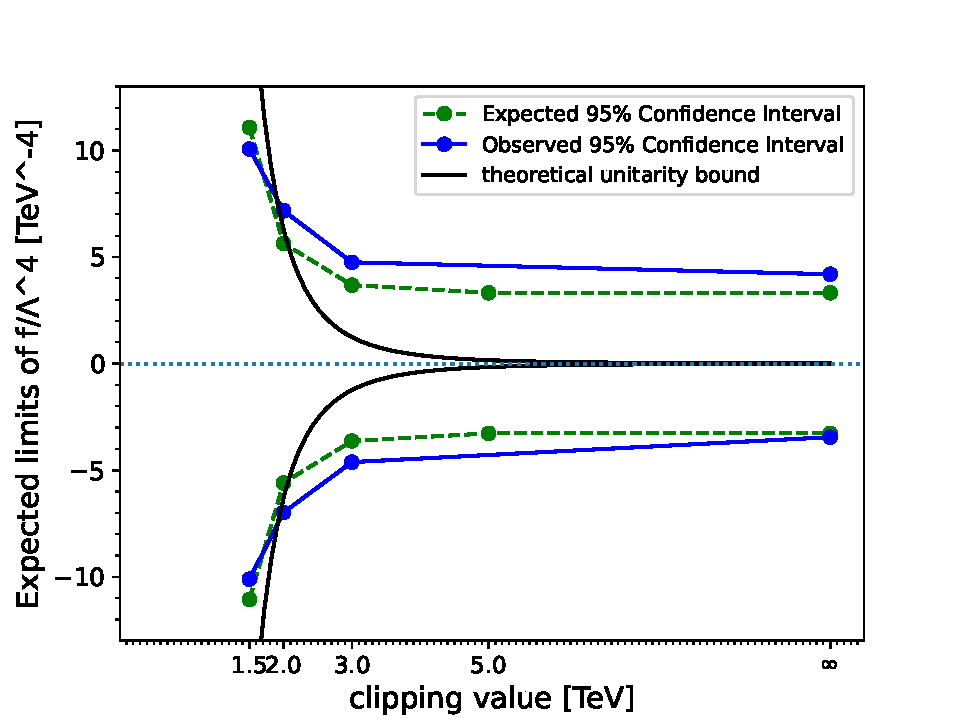
\includegraphics[width=0.45\textwidth]{figures/aQGC/ClippedFS02CI.pdf}
        \caption{Expected limits (green) and observed limits (blue) for 5 clipping points are shown for each Wilson coefficient FT0 (left), FM0 (right), FS02 (middle). The black line is the theoretical unitarity bound.}
        \label{fig:aQGClimits}
\end{figure}